\begin{figure*}[!htb]
	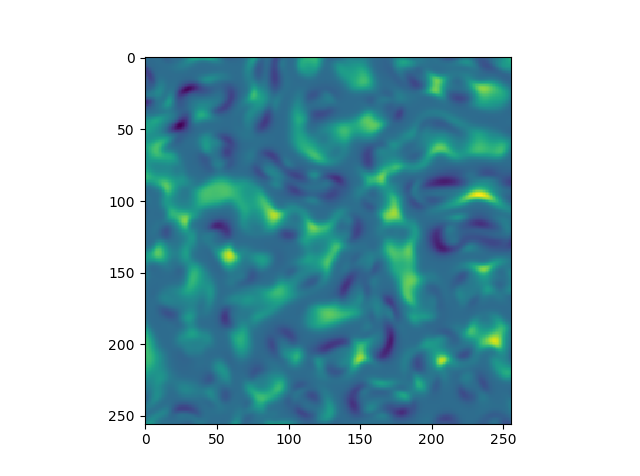
\includegraphics[width=0.33\linewidth]{img/dataset/miranda-viscosity.png}
	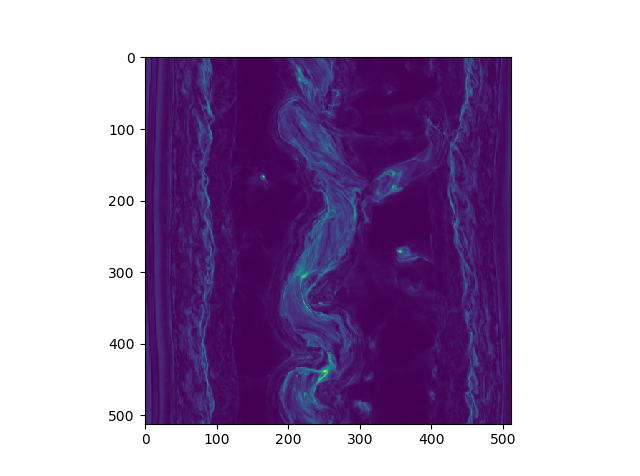
\includegraphics[width=0.33\linewidth]{img/dataset/magnetic.png}
	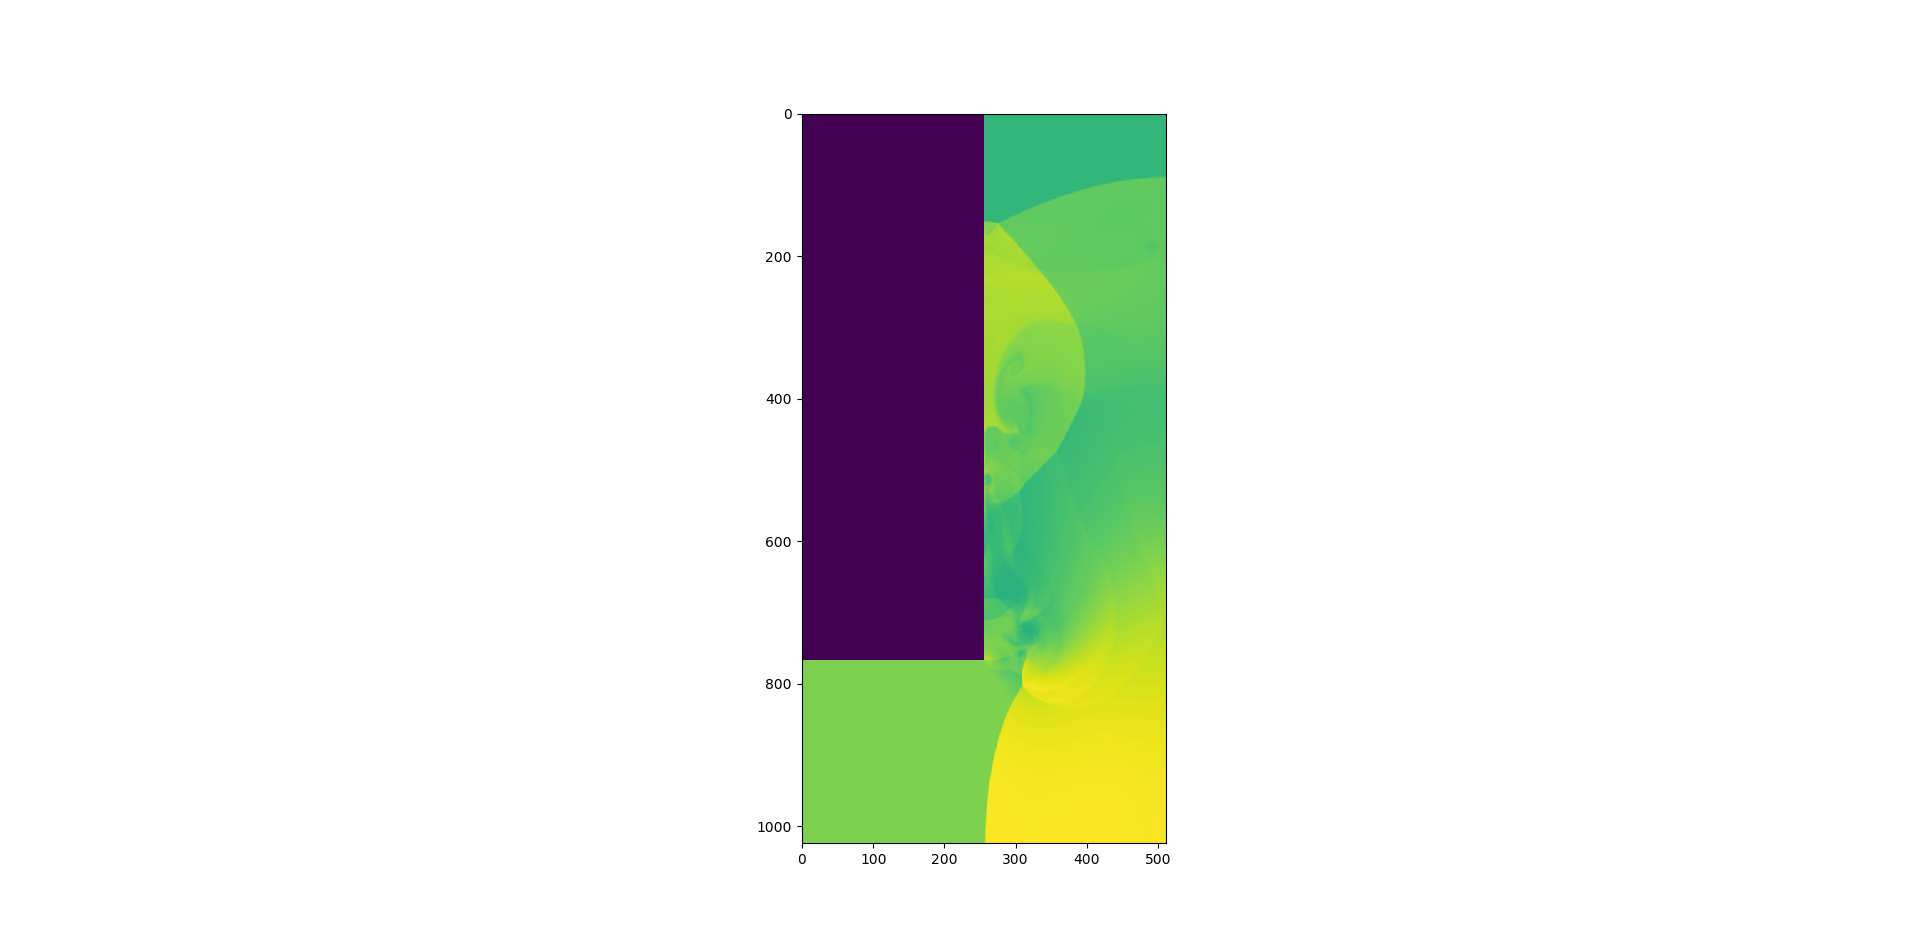
\includegraphics[width=0.33\linewidth]{img/dataset/euler2d.png}
	\caption{Left to right: Miranda viscosity field, magnetic reconnection, Euler 2d sharp front}
	\label{fig:datasets}
\end{figure*}

\section{The need for adaptive-precision and adaptive-resolution data representation}

Traditional data reduction techniques work in either resolution space or precision space exclusively. That is, data is typically reduced by truncation of the last few levels in a multi-resolution hierarchy, or by truncation of lower-ordered bits, but rarely by a mixture of both. It is beneficial, however, to 

\begin{figure}[htb!]
	\centering
	\subcaptionbox{PSNR comparison}
	{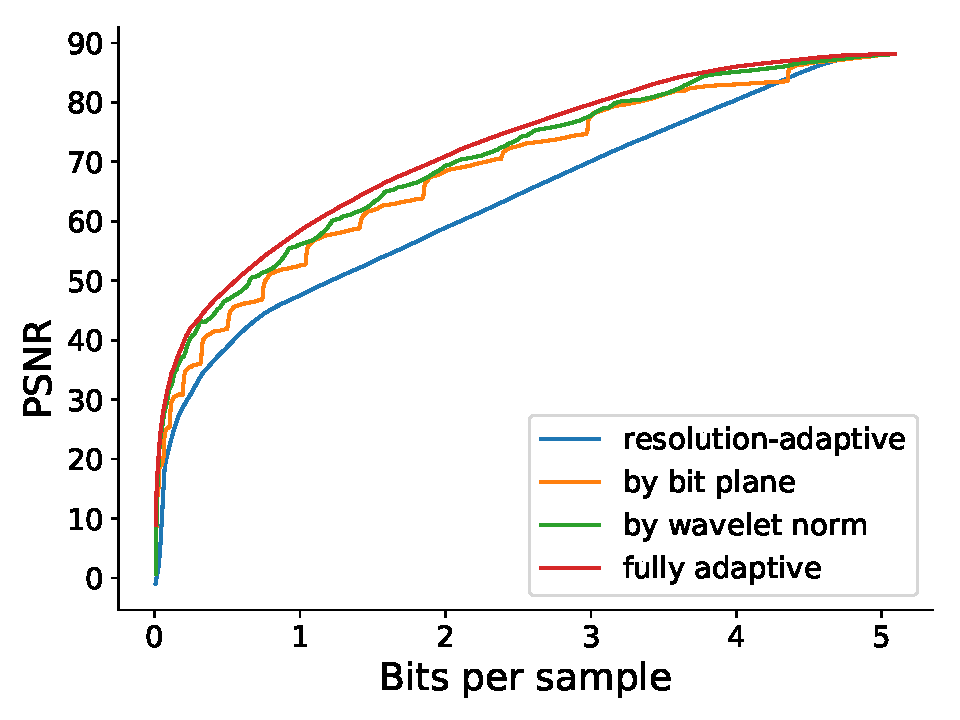
\includegraphics[width=0.8\linewidth]{img/motivation/kflame-oh-motivation.pdf}}
	\subcaptionbox{by bit plane}
	{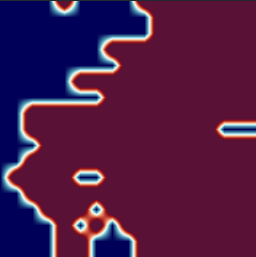
\includegraphics[width=0.21\linewidth]{img/motivation/ERROR-(rmse)-GREEDY-BY-BIT-PLANE-(rmse).png}}
	\subcaptionbox{by level}
	{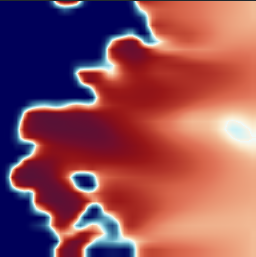
\includegraphics[width=0.21\linewidth]{img/motivation/ERROR-(rmse)-GREEDY-BY-LEVEL-(rmse).png}}
	\subcaptionbox{no constraint}
	{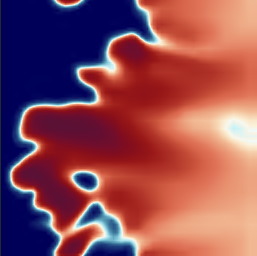
\includegraphics[width=0.21\linewidth]{img/motivation/ERROR-(rmse)-GREEDY-(rmse).png}}
	\subcaptionbox{original}
	{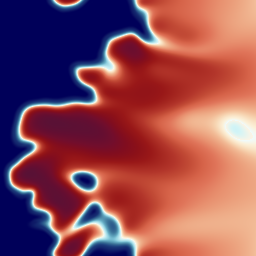
\includegraphics[width=0.21\linewidth]{img/motivation/original.png}}
	\caption {(a) PSNR comparison for three L2 norm-optimized streams: by bit plane, by level, and no constraints. (b, c, d) reconstructed data at 6528 bytes. (e) original data.}
	\label{fig:motivation}
\end{figure}
%Multiresolution data structures or value quantization are commmonly used for data size
%reduction.
%
%However, we show that by both reducing resolution and precision we can achieve lower error
%than by limiting the reduction only to resolution or only to precision. For our experiments
%we use wavelets, where the resolution corresponds to levels, and precision to bitplanes.
%
%For example, we can compute {\em PSNR} for a relatively smooth and uniform dataset, such as Miranda
%viscosity field, and vary only resolution, only precision, or both (\Cref{fig:psnr_traditional_vs_by_norm_viscosity}). Miranda
%dataset is especially useful as the independent stream order does not exhibit any spatial adaptivity and this particular datasets is fairly uniform.

\begin{figure}[htb!]
	\centering
	\subcaptionbox{without skip leading zeros}
	{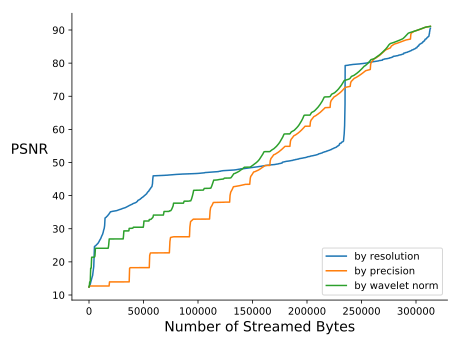
\includegraphics[width=0.4\linewidth]{img/independent/rmse-miranda-viscosity}}
	\subcaptionbox{with skip leading zeros}
	{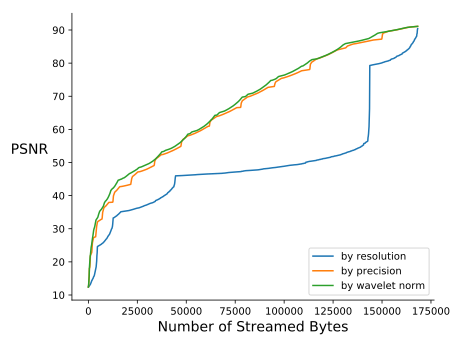
\includegraphics[width=0.4\linewidth]{img/skip-zeros/rmse-miranda-viscosity}}
	\caption {PSNR comparison between three streams: by bit-plane, by level, and by wavelet norm}
	\label{fig:psnr_traditional_vs_by_norm_viscosity}
\end{figure}

%The resolution stream loads level-by-level data with full precision resulting in notable flat regions. These
%regions are coused by the doubling of the samples at each refinement step. Similarly, the precision stream
%shows the similar staircase pattern, but in this case the flat regions are smaller as the bitplane granularity
%is finer than in the resolution stream case. The combination of both these approaches outperform precision
%stream at all times and its finer granularity.

We begin by defining what we mean by resolution and precision. Things to touch on here:

\begin{enumerate}
  \item that we use the (cdf5/3) wavelet transform to generate levels of resolution (subbands) from 2D data
  \item that due to computational contraint, and also because of practical reasons, we group wavelet coefficients into groups of 4x4 pixels
  \item we quantize the data to 16 bits by extracting the maximum exponent
  \item we use negabinary to avoid having to deal with the sign bit in a special way
\end{enumerate}

\textbf{Define} the following streams
\begin{enumerate}
  \item S1: static order, from high to low-order bit planes. Within each bit plane, follow the subband order. This corresponds to simply truncation in practice.
  \item S2: static order, from coarse to fine subbands. Within each subband, each coefficient is streamed in whole. This corresponds to level-of-detail techniques in practice.
  \item S3: static order, but the bits are not coupled in either resolution or precision. The order is determined by the product of $2^i$ (i is the bit plane) and the wavelet basis norm.
  \item S4: greedily-optimized uniform resolution, adaptive precision (i.e all chunks within a subband are streamed together)
  \item S5: uniform precision, adaptive resolution (i.e, all chunks within a bit plane are streamed together)
  \item S6: greedily-optimized, adaptive resolution and adaptive precision 
  \item S7: greedily-optimized, adaptive resolution and adaptive precision, also skip the leading zeros (or equivalently, move the leading zeros to the end of the stream)
\end{enumerate}

\textbf{Figure}: Compare S1, S2, S3, S4, S5, and S6 in PSNR for miranda, viscosity. This figure shows that, first of all (and non-surprisingly) the adaptive streams perform much better than the static ones. Second, it shows among the adaptive ones, except for S7, S6 performs best. Finally S7 gives an empirical bound on the best possible stream for PSNR. (placeholder figure \ref{fig:psnr_traditional_vs_by_norm_viscosity}a)

\begin{figure}[t]
	\centering
	\subcaptionbox{without skip leading zeros}
	{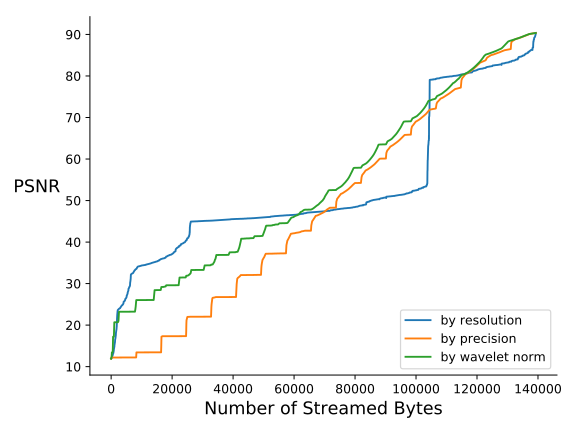
\includegraphics[width=0.4\linewidth]{resources/rmse-miranda-viscosity.png}}
	\subcaptionbox{with skip leading zeros}
	{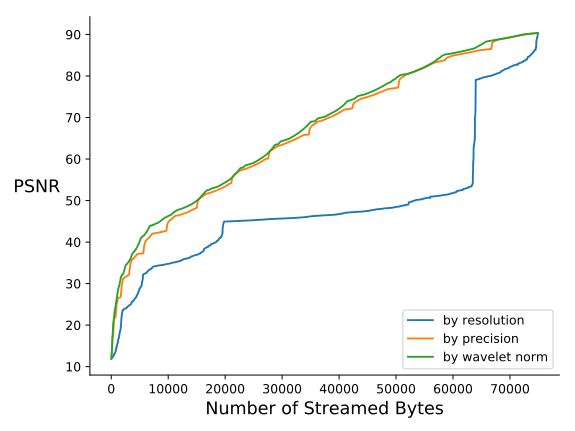
\includegraphics[width=0.4\linewidth]{resources/rmse-miranda-viscosity_slz.png}}
	\caption {PSNR comparison between three streams: by bit-plane, by level, and by wavelet norm}
	\label{fig:psnr_traditional_vs_by_norm_viscosity}
\end{figure}

When compression is used, it avoids streaming the leading zero bits of the wavelet coefficients (figure \ref{fig:psnr_traditional_vs_by_norm_viscosity}b).

In the supplement materials, we show the same plot for the following datasets:
\begin{enumerate}
  \item Miranda viscosity (smooth and uniform)
  \item Kingsnake (noisy and sparse)
  \item Magnetic (tiny narrow lines)
  \item Euler 2D (sharp front)
  \item Enzo u (wide range)
\end{enumerate}

\section{The need for task-specific streams}
From the above two figures we have shown that it is worthwhile to look into streams that are not either simply by bit-plane or by levels. But it is also important that we look into the metric (or the analysis task) at hand to decide what bits to stream. We have shown one example where a stream that works well for one metric (PSNR) does not work well for other metrics (isocontour and histogram) in the previous section. Here we show an example where a PSNR-optimized stream performs poorly compared to an isocontour stream and histogram stream in respective metrics.

Here we show that for isocontour extraction, and for histogram computation, we are better off with other streams.

\textbf{Define} Stream S8 = greedily-optimized for histogram
Figure: histogram error for the following streams: S1, S2, S3, S6, and S8. This figure shows that among the static streams (S1, S2 and S3), the S2 stream performs the best for histogram, in contrast to the case for PSNR above. Comparing the two data-dependent streams S6 and S8, we note that S8 performs better than S6, implying that simply optimizing for PSNR does not result in the best stream for histogram.

\begin{figure}[htb!]
	\centering
	\subcaptionbox{without skip leading zeros}
	{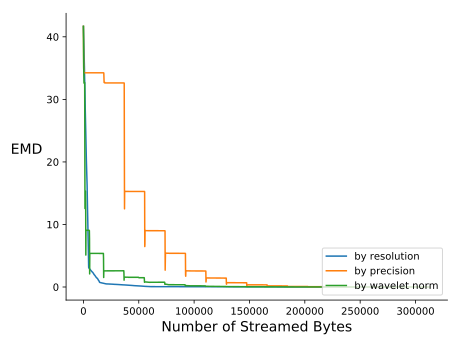
\includegraphics[width=0.4\linewidth]{img/independent/histogram-miranda-viscosity}}
	\subcaptionbox{with skip leading zeros}
	{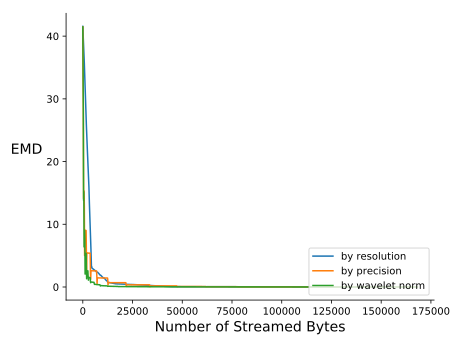
\includegraphics[width=0.4\linewidth]{img/skip-zeros/histogram-miranda-viscosity}}
	\caption {Histogram with earth mover distance (EMD) comparison between three streams: by bit-plane, by level, and by wavelet norm}
	\label{fig:histogram_traditional_vs_by_norm_viscosity}
\end{figure}

\begin{figure}[htb!]
	\centering
	\subcaptionbox{without skip leading zeros}
	{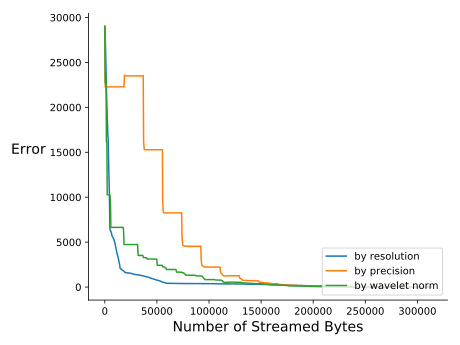
\includegraphics[width=0.4\linewidth]{img/independent/isocontour-miranda-viscosity}}
	\subcaptionbox{with skip leading zeros}
	{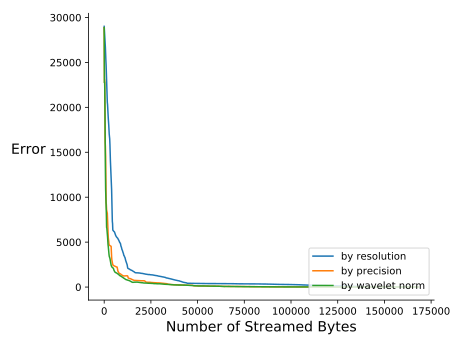
\includegraphics[width=0.4\linewidth]{img/skip-zeros/isocontour-miranda-viscosity}}
	\caption {Isocontour ($h = 0.0634$) comparison between three streams: by bit-plane, by level, and by wavelet norm}
	\label{fig:isocontour_traditional_vs_by_norm_viscosity}
\end{figure}

\begin{figure}
  \centering
  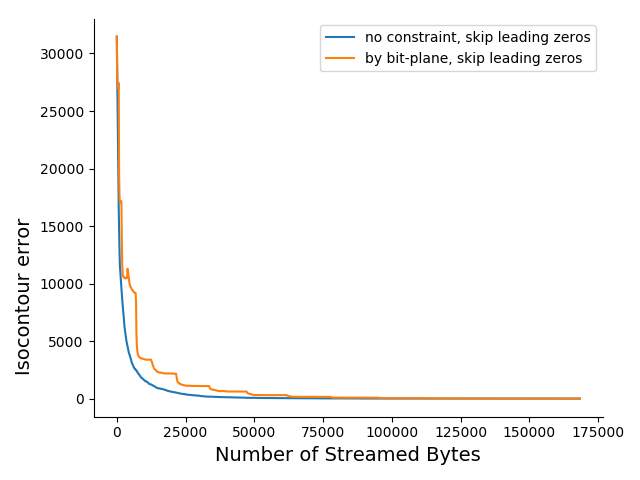
\includegraphics[width=0.8\linewidth]{resources/isocontour-error-by-bit-plane-viscosity.png}
  \caption {By bit-plane isocontour comparison versus no constraints for viscosity, isoval=-0.005}
  \label{fig:by_bit_plane_isocontour}
\end{figure}
